\subsection{Radar Simulations} \label{compvis_radarsims}

    \subsubsection{Introduction and Physical Principles} \label{rory_radar_principles}
    
        As outlined in Section \ref{simulation_justification}, the limited diversity of the radar dataset necessitates physics-driven simulations to replicate the noise and clutter encountered in real-world environments. These simulations aim to validate the CNN’s robustness to physical processes that degrade B-scan clarity, ensuring reliable performance under operational conditions.
    
        The electromagnetic phenomena governing radar losses are:
        \begin{itemize}
        
            \item \textbf{Antenna losses}: Mismatch losses (approximately −1 dB \cite{daniels2005gpr}), and efficiency losses (excluded as secondary to subsurface effects).
            
            \item \textbf{Transmission losses}: Signal attenuation from reflections at air-soil and soil-air interfaces.
            
            \item \textbf{Material losses}: Frequency-dependent attenuation within heterogeneous soils.
            
            \item \textbf{Scattering losses}: Arising from subsurface inhomogeneities in soil composition, and soil surface roughness.
        
        \end{itemize}
        
        To model these effects, finite-difference time-domain (FDTD) simulations were conducted using \textit{gprMax} \cite{warren2016gprmax}, an open-source framework for solving Maxwell’s equations in 3D geophysical media. This approach captures full-wave electromagnetic behaviour, including wave propagation, reflection, and attenuation, while explicitly accounting for soil heterogeneity. The inclusion of surface roughness is not considered in this report, as for the purposes of validating the CNN-driven detection framework, modelling of subsurface heterogeneity suffices to ensure robustness to clutter. This is however a significant contribution to the clutter observed in an operational GPSAR system, and future work should consider this aspect that has been overlooked here.
     
    
    
    \subsubsection{gprMax Implementation}

        \paragraph{Radar}
        
             The source/receiver configuration follows recommendations provided by Huirui (see Section XX) and employs a Ricker waveform as the excitation signal. The Ricker waveform is widely used in GPR and seismic applications for its clear central frequency and well‐defined bandwidth properties \cite{dummyRef2}. A central frequency of 1.5\,GHz was chosen, as it provides a good compromise between penetration depth and resolution—even in moderately moist soils where deeper penetration is required. The transmitter and receiver are modelled as Herzian dipole antennas 10cm from the surface of the soil, and separated from each other by 2cm. B-scans are produced by taking successive A-scans while moving the source and receiver in 4\,mm increments from left to right across the simulation domain
    
        \paragraph{Domain}

            The simulated computational domain spans $0.8\times 0.3\times0.02$\,m ($x\times y\times z$), representing a quasi-2D space. The domain is discretised into cubic elements of side length 0.002\,m , 100 times smaller than the wavelength of the radar pulse. Two thirds of the domain is occupied with soil, and the rest with air. A circular landmine with radius 5\,cm was buried with its centre 0.1\,m below the surface of the soil, and was modelled as a perfect electric conductor (PEC), representative of a metallic landmine.


        \paragraph{Boundary Conditions}
        
            Perfectly matched layers (PMLs) are used as obsorbing boundary conditions on all sides of the domain, to mimick an open boundary. The source and receiver were placed more than 20 cells away from the PML regions to avoid erroneous interference. Each simulation was run for 5$\times$10$^{\text{-9}}$\,s, enough to capture all the relevant electromagnetic phenomena.

        
    
    \subsubsection{Heterogeneous Soil Model}
    
        A realistic simulation of electromagnetic wave propagation necessitates an accurate representation of the subsurface. In this work, the heterogeneous soil is modelled using the Peplinski model, which characterises soil dielectric properties based on sand fraction, clay fraction, bulk density, sand-particle density and volumetric water fraction range, over a frequency range of 1-18\,GHz. To capture the natural spatial variability, a fractal generation technique is employed \cite{dummyRef5}. This method replicates the self-similar patterns observed in natural soils over multiple scales, thereby enhancing the fidelity of the simulation, and accurately accounting for the heterogeneity in the soil. Detail of the Peplinski soil model, and the fractal generation technique can be found in \cite{warren2016gprmax}. 

        \paragraph{Soil Parameters}

            For the simulation to give realistic results, it is initialised with accurate soil parameters for Ukraine. Ukraine is mostly covered with the very fertile Chernozem soil \footnote{\url{https://www.britannica.com/place/Ukraine/Soils}}, the properties of which were taken from \cite{suleymanov2021chernozem}, and are summarised here.

            \begin{table}[htbp]
              \centering
              \caption{Properties of Chernozem Soils}
              \begin{tabular}{@{} l l @{}} 
                \toprule
                \textbf{Property} & \textbf{Value} \\
                \midrule
                Clay fraction & $\sim 30\%$ \\
                Sand fraction & $\sim 70\%$ \\
                Bulk density & $\sim 1.4$ g/cm$^3$ \\
                Sand particle density & $2.65$ g/cm$^3$ \\
                Volumetric water fraction range & $1\% - 10\%$ \\
                \bottomrule
              \end{tabular}
            \end{table}
    
        \begin{figure}[htbp]
            \centering
            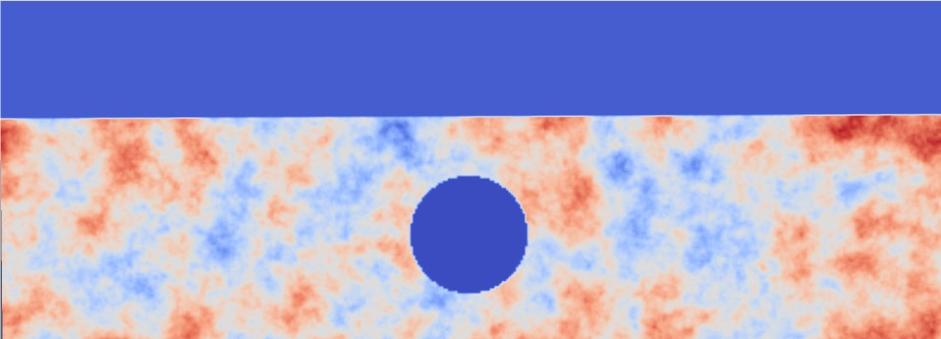
\includegraphics[width=0.8\textwidth]{figs/Rory/radar_domain.pdf}
            \caption{Simulation domain viewed in ParaView.}
            \label{fig:radar_domain}
        \end{figure}
        \footnote{\url{https://www.paraview.org/}}
    
    \subsubsection{Results and Validation}
    
        Figure~\ref{fig:original_bscan} shows the simulated radar responses, illustrating the backscattered signatures generated by the presence of a buried landmine. These responses have been compared with real GPR data obtained from controlled field experiments \cite{dummyRef7}, demonstrating reasonable agreement. However, computational limitations restrict the number of simulations that can be feasibly run, and the current model assumes a simplified environment with flat ground, no foliage, and an absence of puddles or other surface irregularities. These factors may contribute to discrepancies between simulated and real-world data.
    
        \begin{figure}[htbp]
            \centering
            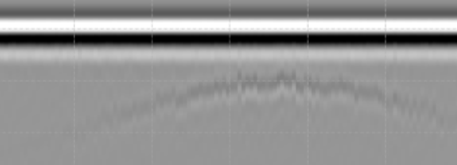
\includegraphics[width=0.8\textwidth]{figs/Rory/sim_bscan_cropped.png}
            \caption{Raw simulated B-scan (no digital enhancement)}
            \label{fig:original_bscan}
        \end{figure}
    
    \subsubsection{Data Augmentation}
    
      Running these simulations is computationally intensive, so one should make the most of each simulation performed. From this one simulation, multiple image augmentations were applied, each representing a physical process. The transforms considered were stretching (representing different soil properties and mine shape), cropping (representing Bscans that did not capture the whole mine) and adding Gaussian blur (representing greater attenuation of high frequencies due to different soil properties), and combinations of these. Contrast limited adaptive histogram equalisation (CLAHE) \footnote{\url{https://en.wikipedia.org/wiki/Adaptive_histogram_equalization}} is also applied to the original image regardless of the other transformations applied, to enhance the image clarity whilst keeping the contrast manageable. When these transformations are applied to the simulated Bscan, a dataset of 90 images is generated. This is sufficient to test whether the pre-trained CNN (Section \ref{compvis_implementation}) is robust to heterogeneous soil properties and other physical loss phenomena.
        
        \begin{figure}[htbp]
          \centering
        
          \adjustbox{valign=c}{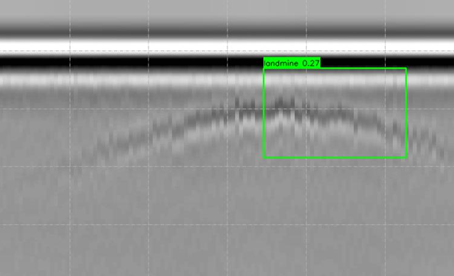
\includegraphics[width=0.32\textwidth]{figs/Rory/sim_bscan_clahe_detection_cropped.png}}
          \hfill
          \adjustbox{valign=c}{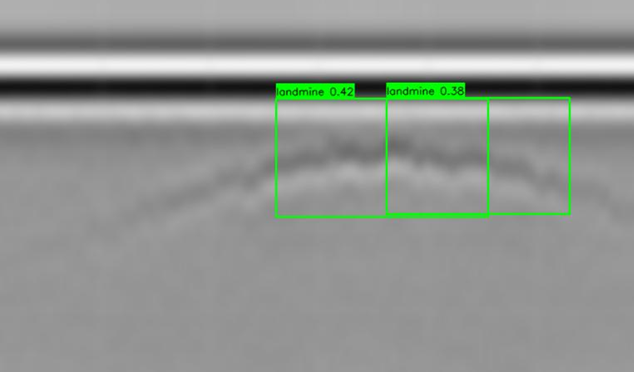
\includegraphics[width=0.32\textwidth]{figs/Rory/sim_bscan_clahe_detection_blur_cropped.png}}
          \hfill
          \adjustbox{valign=c}{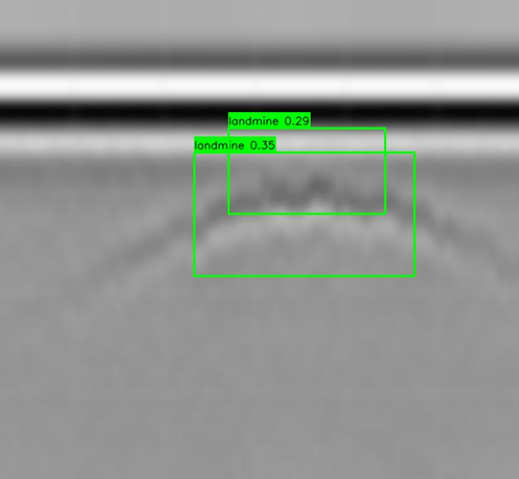
\includegraphics[width=0.32\textwidth]{figs/Rory/sim_bscan_clahe_detection_blur_stretched_cropped.png}}
        
          \caption[Comparison of simulated B-scans under different pre-processing steps]{Comparison of simulated B-scans under different pre-processing steps. 
          (a) Simulated B-scan with CLAHE applied. 
          (b) Simulated B-scan with CLAHE and Gaussian blur applied. 
          (c) Simulated B-scan with CLAHE, Gaussian blur, and a vertical stretch applied. 
          In each case, the bounding boxes from the pre-trained CNN in Section \ref{compvis_implementation} are visible, with the corresponding numerical confidence level.}
          \label{fig:sim_bscan_comparison}
        \end{figure}
        
    
    \subsubsection{CV Results}
    
        The augmented radar data were subsequently analysed using the pre-trained CNN (Section \ref{compvis_implementation}) to evaluate the robustness of the model to the physical loss processes described in Section \ref{rory_radar_principles}. Precision and recall metrics were calculated on the augmented dataset, with the results summarised in Table~\ref{tab:cv_results}, indicating that the combined approach of GPSAR and SOTA CV techniques is promising for practical landmine detection. In particular it is noted that we can achieve a high precision with moderate recall with the GPSAR sensor, and that the CNN, although trained on a very homogenous 'clean' dataset generalised well to a more varied dataset from high-order simulations that directly model the noise processes (which we have argued in SEC XX is very important).

        \begin{table}[htbp]
          \centering
          \caption{Augmented Simulation Bscan Results}
          \begin{tabular}{@{} l l @{}} 
            \toprule
            \textbf{Metric} & \textbf{Value} \\
            \midrule
            Number of actual landmines & 90 \\
            Number of true positive predictions & 75 \\
            Number of false positive predictions & 7 \\
            Number of false negative predictions &  15\\
            \midrule
            \textbf{Precision} &  \textbf{91.5\%}\\
            \textbf{Recall} & \textbf{83.3\%}\\
            \bottomrule
          \end{tabular}
        \end{table}       
        
        \paragraph{Summary} These findings show that a GPSAR sensor coupled with an open-source CNN detection algorithm demonstrates great feasibility for reliably identifying buried landmines across diverse terrains. This is validated by achieving high precision (91.5\%) on a diverse dataset comprising simulated radar scans in a heterogeneous Ukrainian soil, despite being trained on a small dataset with limited variability. The system's current performance likely represents a lower bound, and it is expected that an improved system trained on a larger dataset of more varied radar scans from experimentation or simulation, would yield greater precision, potentially above 95\%. Overall, this system offers a highly maintainable and effective solution, that can improve as more context specific training data becomes available.